\begin{figure}[p]
\centering
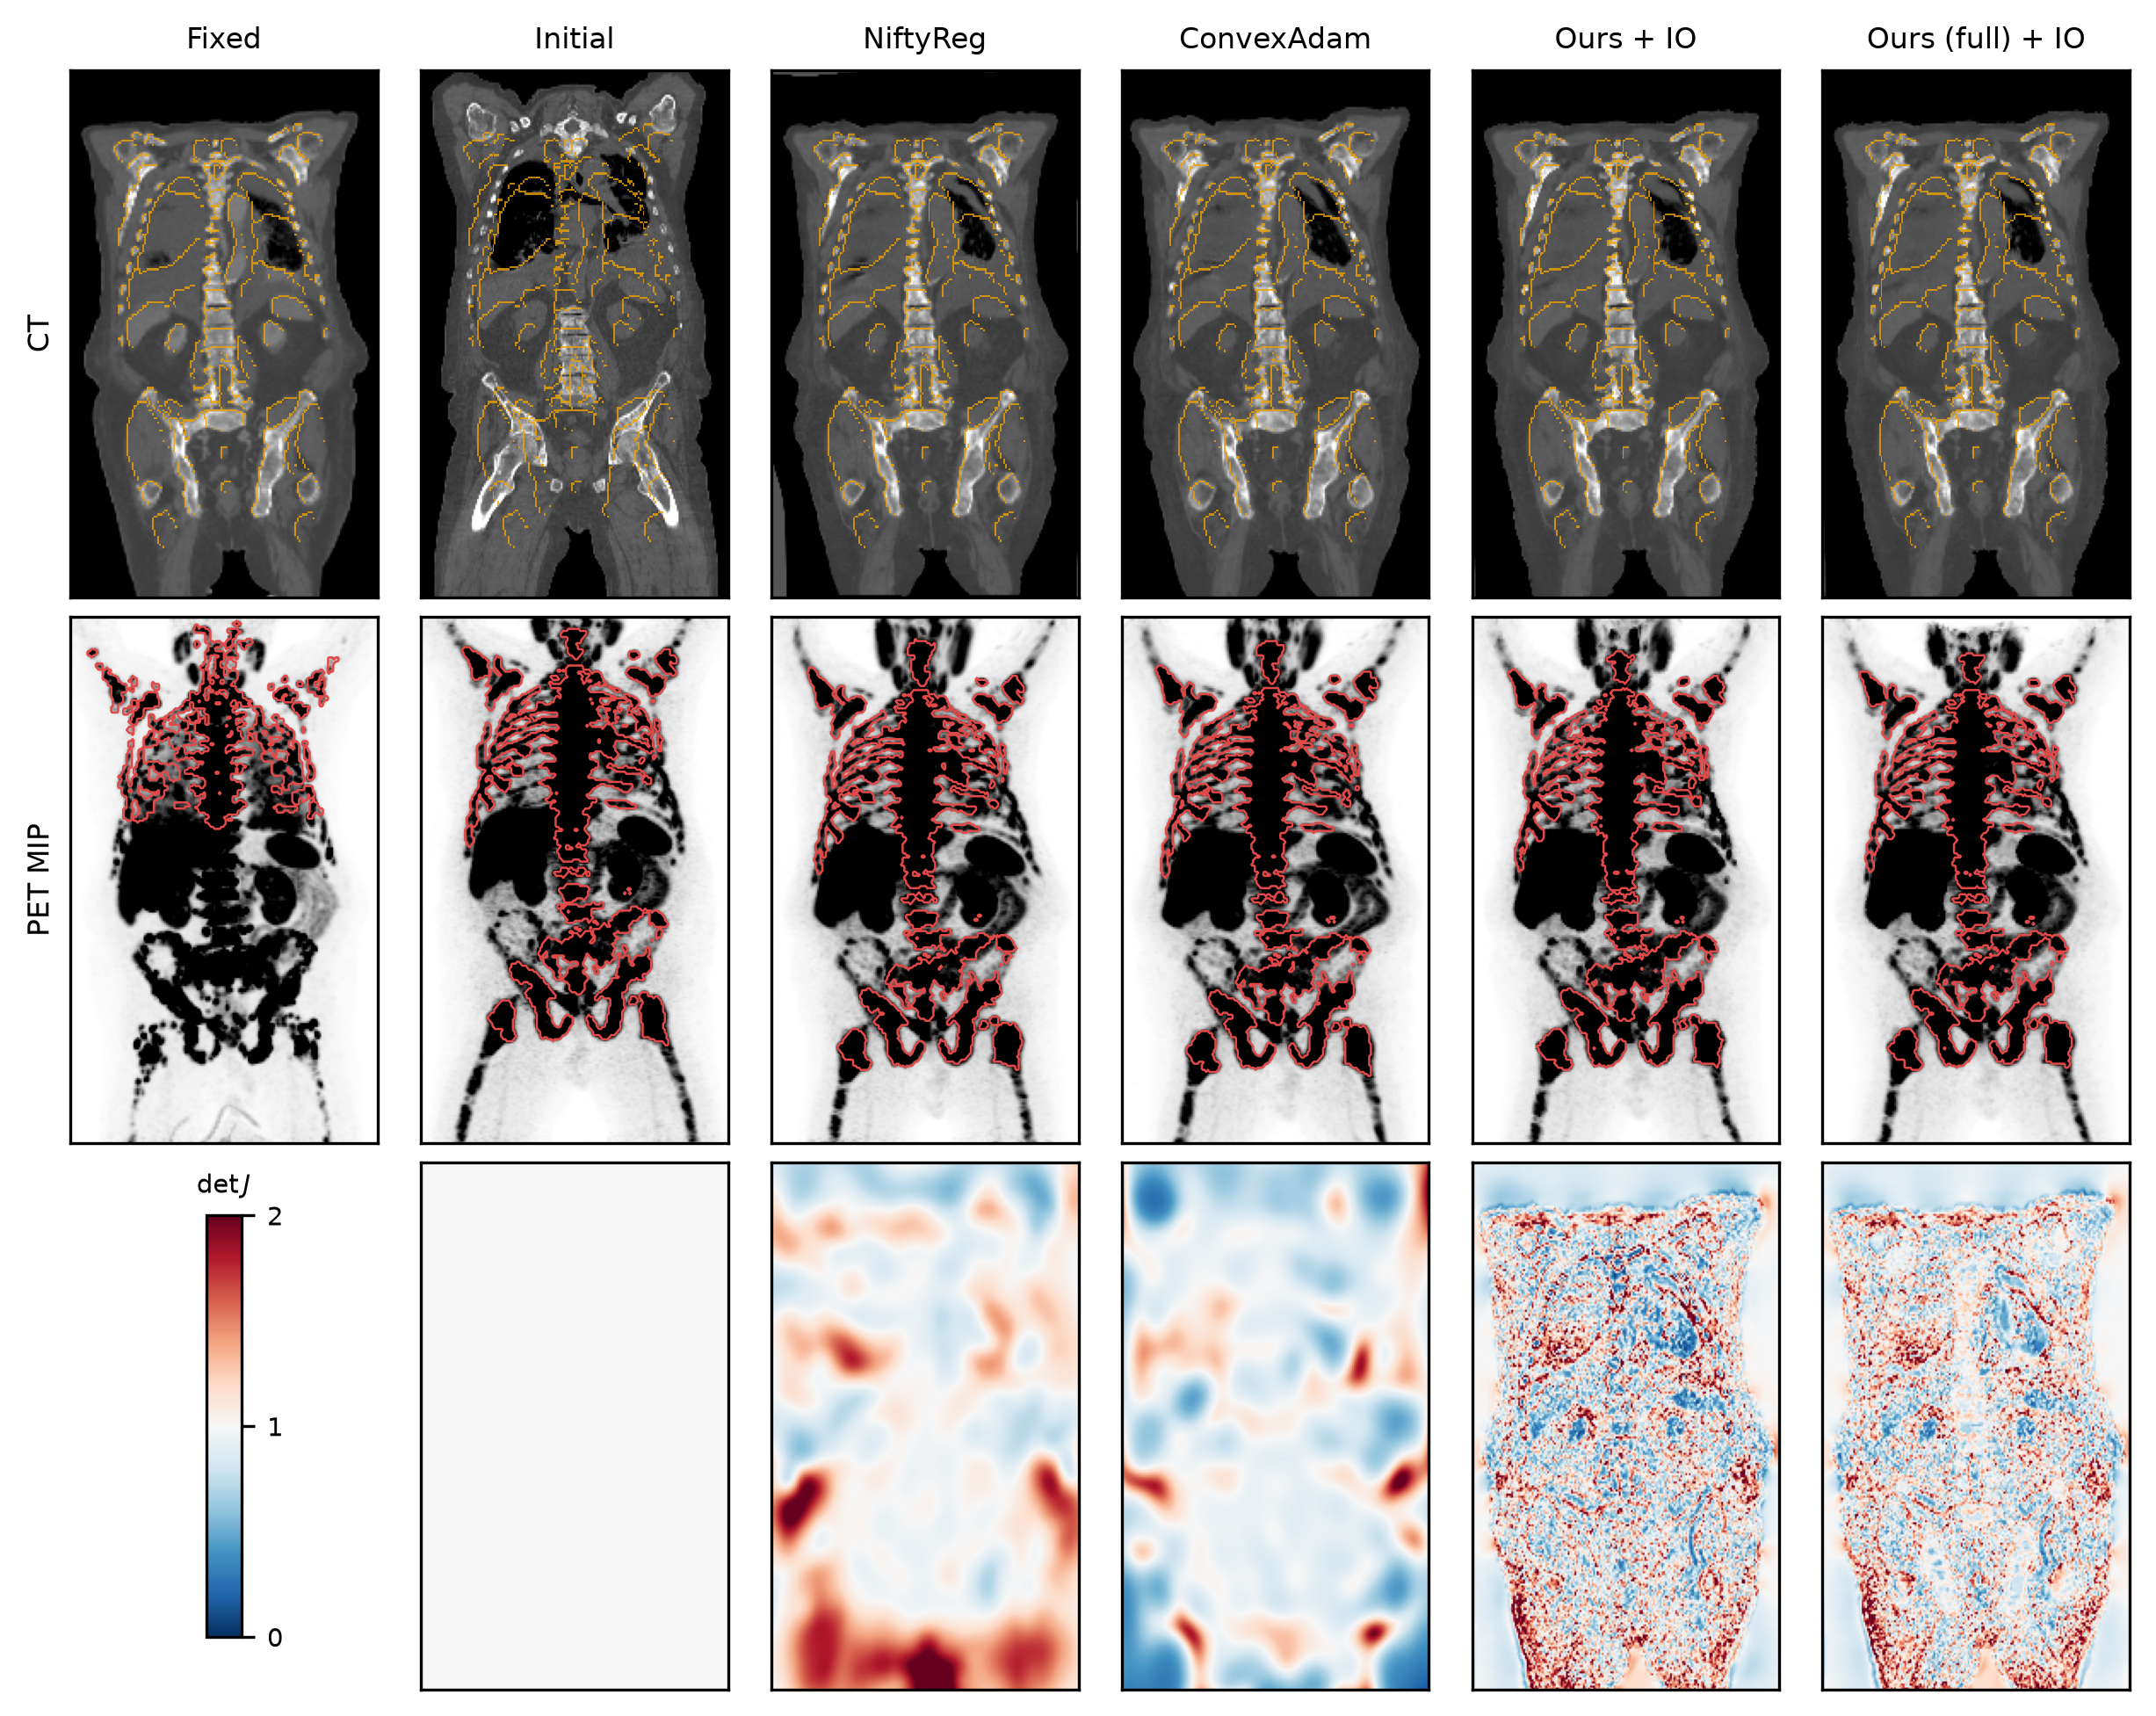
\includegraphics[width=\textwidth]{figures/qualitative.png}
\caption{Anatomical alignment example from the test set, registered by our method (PET-preservation and rigidity losses only in instance optimization [IO]); one coronal slice.
 Patient 0146 was selected for its large between-image change in lesion volume (2400 voxels at baseline and 24\,191 at follow-up).
 The example illustrates anatomical alignment and deformation.
 (a)~Fixed and (b)~moving CT images overlaid with the corresponding PET images (SUV 0--8, 35\,\% opacity) and provided lesion contours (red).
 (c,~d)~Fixed CT image (green) overlaid with the moving CT image (magenta) before~(c) and after~(d) registration; gray where they agree.
 (e,~f)~Organ labels that differ before~(e) and after~(f) registration: green where the fixed image has a label that the moving image lacks there, magenta where only the moving image is labeled; bright, medium, and dark shades for bones, organs, and muscles.
 (g)~Jacobian determinant of the fixed-to-moving transformation: white is volume-preserving (1), blue is below 1 and red is above 1; changes in the displayed warped anatomy have the opposite direction.
 (h)~Warped moving CT image overlaid with the corresponding PET image and warped lesion contours.}
\label{fig:qualitative}
\end{figure}
